%%%%%%%%%%%%%%%%%%%%%%%%%%%%%%%%%%%%%%%%%%%%%
%INTRODUCTION
%%%%%%%%%%%%%%%%%%%%%%%%%%%%%%%%%%%%%%%%%%%%%

\section{An Introduction to plant pathogenic \textit{Fusarium} species}




\subsection{\textit{Fusarium} of banana}


\subsubsection{Isolates collected by \acl{tnau}, India}

This chapter presents the assembly and analysis of the genomic characteristics of \textit{Fusarium} isolates (SY-2, S6, S16, and S32) obtained from Cavendish banana plants by collaborators at \acl{tnau}, India (\acs{tnau}). Taxonomic identity and genetic diversity are assessed and suggest that there is a potentially novel species of \textit{Fusarium} infecting banana. Of the isolates sequenced, S6 is a \ac{Focub} \ac{r1} isolate, while SY-2, S16 and S32 belong to the \textit{F. fujikuroi} species complex. Phylogenetic analysis and \ac{sixg} profiling supported these classifications. Isolates SY-2 and S16 are reported as \textit{Fusarium saccahri} isolates, S32, however, represents a novel clade within the \textit{F. fujikuroi} complex. It is important to note, however, that bacterial contamination with \textit{Stenotrophomonas} species was detected in S6 and S32 isolates, warranting future studies to confirm this potentially novel taxon.

%%%%%%%%%%%%%%%%%%%%%%%%%%%%%%%%%%%%%%%%%%%%%
%METHODS
%%%%%%%%%%%%%%%%%%%%%%%%%%%%%%%%%%%%%%%%%%%%%

\section{Materials and Methods}
\subsection{Phenotyping and genotyping data supplied by \acl{tnau}.}

Collaborators a \ac{tnau} aimed to assess the diversity of the \ac{Focub} in Tamil Nadu and to understand the genetic and molecular basis of resistance against \ac{Focub} in banana through next-generation genomics. A survey was conducted in various banana-growing areas of Tamil Nadu to record symptoms of wilt in different banana cultivars. 

Samples displaying symptoms of \textit{Fusarium} wilt, including the \ac{Focub4} susceptible Cavendish banana variety 'Grande Nain' were collected from the field, and the pathogen was isolated and cultured in the laboratory. Among the collected samples, isolates SY-2, S6, S16, and S32 were chosen for further analysis. DNA extraction and PCR amplification were performed to confirm the isolates' identity. 

The isolated strains, S6, S16, and S32, exhibited severe disease symptoms when inoculated into tissue-cultured 'Grand Naine' banana plants and were classified as highly virulent. PCR amplification using race 4-specific primers confirmed that SY-2, S6, S16, and S32 were \ac{Focub4} isolates, capable of infecting Cavendish banana (Work conducted at \ac{tnau} is summarised in Appendix ). Isolates SY-2, S6, S16, and S32 were sequenced using the \textcolor{red}{WHICH PLATFORM, WHAT STATS CAN WE EXTRACT HERE?}.\footnote{\textcolor{red}{Due to communication challenges with collaborators at TNAU, we have not been able to establish the extraction protocol used to produce the DNA used for sequencing.}}

\subsection{Analysis of Raw Read data from TNAU isolates}

The raw Illumina paired-end reads for the \textit{Fusarium} isolates SY-2, S6, S16, and S32, which are reported to be highly virulent on Cavendish banana, were supplied by collaborators at \ac{tnau}. Following FastQC (Version 0.11.8) (Andrews, 2010) analysis, raw reads were mapped to \ac{Focub4}  isolate UK0001 (Warmington, \et 2019) reference quality genome using BOWTIE2 (version 2.4.5) (Langmead and Salzberg, 2012). Due to poor mapping rates for some isolates, 1000 raw reads were extracted from each \ac{tnau} isolate and searched using \ac{ncbi} web \ac{blast} (Nih.gov, 2014). 
Raw reads were then mapped to \ac{Focub1} isolate 160527(Asai, \et 2019), as well as \textit{Fusairum sacchari} isolate FS66 (Cui \et 2021). Isolates S6, S16 and S32 were also mapped to a reference quality \textit{Stenotrophomonas maltophilia} isolate NCTC10258 genome (GCA\_900475405.1) 

\subsection{Genome Assembly and Annotation}

\subsubsection{\textit{De novo Assembly}}
A \textit{de novo} assembly was generated for the \ac{tnau} isolates using SPAdes (v3.14.1) following FastQC (Version 0.11.8) (Andrews, 2010) analysis. SPAdes is routinely employed when generating \textit{Fusarium} genomes (see: Armitage, \et 2018; Hudson \et 2020, Tanaka, \et 2022). A custom Python script was developed to remove sequences with <25\% GC content from the assembly (Appendix ~\ref{apx:gcTrimmer.py}). For assemblies with high levels of contamination (S32, S6), only reads mapping to reference genomes were used to generate \textit{de novo} assemblies.

\subsubsection{Contamination Analysis and Quality Assessments}
Blobtools (v1.1.1) (Laetsch and Blaxter, 2017) was used for the taxonomic partitioning of the assemblies. The \ac{tnau} assemblies were searched against the \ac{ncbi} nt database using BLASTN and the paired-end raw reads were aligned to each of the assemblies using BOWTIE2 (version 2.4.5). Taxonomic hits were ranked at the species level using default BolbTools settings. To extract contigs that have been assigned to a non-\textit{Fusarium} genus by BlobTools, the BlobTools output json file was filtered using blobtools view, with the -r species flag provided. Contigs assigned to a \textit{Fusarium} species or "no-hit" were then extracted and saved in a separate text file. The blobtools seqfilter command with the default settings was then used to extract contigs that had been assigned to \textit{Fusarium} or had "no-hit" (script available in Appendix ~\ref{apx:ContamFilter}).

The quality and completeness of the assembled genomes were estimated using \ac{busco} with the data set hypocreales\_odb10 (Manni \et 2021). The raw reads were mapped back to the assemblies and a Qualimap assessment was conducted (García-Alcalde \et 2012). Quast (v5.0.2) (Gurevich \et 2013) was used to estimate assembly quality statistics. 

\subsubsection{Repetitive Element Identification}

Repetitive elements were identified in each contaminant-filtered assembly using RepeatModeler (version 2.0.4) ((Flynn \et 2020)) including the -LTRStruct option. Once models had been generated, they were combined with the RepeatMasker default fungal database to create a custom repeats library for each isolate. RepeatMasker (version 4.1.5) (Smit, Hubley and Green, 2010) was then used to soft-mask each assembly. 

\subsubsection{Genome Annotation}
Following masking, the \ac{tnau} genomes were annotated using MAKER textcolor{red}{[VERSION AND CITATION]}. As no RNA sequencing data were available for these isolates, a reference proteome set was generated using the \ac{ncbi} RefSeq nr database, using the search term "Fusarium AND srcdb\_refseq[PROP]" with the protein option selected. MAKER was run using textcolor{red}{[PARAMETERS - Explain that it was trained multiple times and snap was included!]}

\subsection{Identification of pathogen-specific features.}

\subsubsection{Ortholog analysis?}

\subsubsection{SIX gene searches – remove coverage and ident thresholds.}
\Acp{sixg} from Fol isolate Fol007 were downloaded from the GenBank and were used as a query in a BLASTX search (1e-6 cut-off, 50\% identity and 70\% coverage threshold) against the genomes to check the presence/absence of \acp{sixg} in all reading frames. A binary data matrix indicating presence (“1”) or absence (“0”) was generated using the BLASTX hit data and a heatmap is generated using the R package, Pheatmap.

\subsubsection{\textit{Mimp} identification approach.}

\subsubsection{EffectorP analysis of proteome through SignalP and EffectorP}


\subsection{Phylogenetic Analysis of \ac{tnau} isolates}\label{chap2:phylogeny}

The common Fusarium genetic barcodes \ac{tef} and \ac{rbp2} were used to generate phylogenies (Edel-Hermann and Lecomte, 2019). Briefly, a \ac{tef} and \ac{rbp2} sequence database were compiled using available reference sequences from the \ac{ncbi} database. Homologs of each barcode were identified in each assembly in our database (See section:~\ref{chap3:fusariumdb}) using BLASTN (1e-\textsuperscript{6} cut-off). The locations of hits with greater than 70\% identity and 90\% coverage were recorded, and the sequence within this region was extracted using Samtools (Version 1.15.1). The \ac{tef} and \ac{rbp2} regions from each genome were concatenated into a single FASTA file for each barcode. MAFFT (Katoh \et 2019) was used to construct a multiple sequence alignment adjusting the direction according to the first sequence to ensure correct alignment and any overhanging regions were trimmed manually. IQ-TREE (Version 2.2.0.3) (Nguyen \et 2015) was used to infer a maximum-likelihood phylogeny using the ultrafast bootstrap setting for 1000 bootstrap replicates and was visualised using iTOL (Letunic and Bork, 2021). 



%%%%%%%%%%%%%%%%%%%%%%%%%%%%%%%%%%%%%%%%%%%%%
%RESULTS
%%%%%%%%%%%%%%%%%%%%%%%%%%%%%%%%%%%%%%%%%%%%%

\section{Results}
\subsection{Phenotyping and genotyping data supplied by TNUA.}

The collaborative study undertaken by researchers at \acs{tnau} aimed to investigate the diversity of \ac{Focub} in Tamil Nadu and explore the mechanisms of resistance against this pathogen in banana using advanced genomics techniques. The initial step involved a comprehensive survey conducted across various regions in Tamil Nadu to document and assess wilt symptoms in different banana cultivars.

Samples exhibiting symptoms of \textit{Fusarium} wilt, including the widely grown 'Grande Nain' Cavendish banana variety susceptible to \acs{Focub4}, were collected. The isolated pathogen was successfully cultured under controlled laboratory conditions and Koch's postulates confirmed. 

Confirmatory tests based on DNA extraction and PCR amplification were carried out to validate the identity of the isolates. Intriguingly,  isolates S6, S16, and S32 displayed a robust ability to induce severe disease symptoms upon inoculation into tissue-cultured 'Grand Naine' banana plants, and were classified as highly virulent \textcolor{red}{[CAN I USE ONE OF THEIR IMAGES HERE?]}.

Further investigations using race 4-specific primers in PCR amplification confirmed that the isolated S6, S16, and S32 strains belonged to the \acs{Focub4} group, demonstrating their capacity to infect Cavendish banana. As a consequential step, the isolates underwent sequencing. However, specific details such as the sequencing platform and statistical insights derived from the sequencing data remain pending due to ongoing communication challenges with \ac{tnau} collaborators.

\subsection{Analysis of Raw Read data from TNAU isolates}

Raw read mapping of the SY-2, S6, S16, and S32 to the \ac{Focub4} UK0001 assembly, produced a 54.11\%, 8.72\%, 53.81\%, and a 15.69\% alignment for all raw reads, respectively (~\ref{tab:RawReadMapping}). 

Due to the low alignment rates, unmapped reads were extracted and a random subset of 1000 reads per isolate were searched using NCBI web BLAST (Nih.gov, 2014). For isolates S6 and S32, the majority of hits with >90\% coverage and identity were for \textit{Stenotrophomonas} species, particularly \textit{Stenotrophomonas maltophilia}. Further, the raw S6 and S32 reads show a similar GC\% to the \textit{S. maltophilia }reference genome assembly (GCA\_900475405.1) (S6=63\%, S32=61\%, \textit{S. maltophilia} reference=66.5\%). For isolate S16, the majority of hits for unmapped reads with >90\% coverage and identity against the NCBI database were for \textit{Fusarium fujikuroi}. Isolates S6, S16 and S32 were also mapped to a reference quality \textit{Stenotrophomonas maltophilia} genome due to the high number of blast hits. 

Approximately 50\% of raw reads from isolates S6 and S32 mapped to the \textit{S. maltophilia} reference (Table ~\ref{tab:RawReadMapping}). Raw reads from isolate S16 only had a 0.01\% mapping rate to the \textit{S. maltophilia} reference. Raw reads from isolates S6 and S32 had a 5.24\% and 22.49\% mapping rate to the \textit{F. sacchari} reference, respectively, whereas 68.65\% of the raw reads from isolate S16 and 93.96\% of the raw reads from the SY-2 isolate mapped to the \textit{F. sacchari} reference.

% Please add the following required packages to your document preamble:
% \usepackage{booktabs}
% \usepackage{multirow}
% \usepackage{graphicx}
\begin{table}[h!]
\caption[Overall alignment rate of all raw reads from each TNAU isolates to fungal and bacterial reference species]{{\textbf{Overall alignment rate of all raw reads from each TNAU isolates to fungal and bacterial reference species.}} Overall alignment rate determined by Bowtie2 (version 2.4.5). Reference assemblies were downloaded from GenBank: \ac{Focub4} isolate UK0001 (\href{https://www.ncbi.nlm.nih.gov/datasets/genome/GCA_007994515.1/}{GCA\_007994515.1}), \ac{Focub1} isolate 160527 (\href{https://www.ncbi.nlm.nih.gov/datasets/genome/GCA_005930515.1/}{GCA\_005930515.1}), \textit{Fusairum sacchari} isolate FS66 (\href{https://www.ncbi.nlm.nih.gov/datasets/genome/GCA_017165645.1/}{GCA\_017165645.1}), \textit{Stenotrophomonas maltophilia} isolate NCTC10258 (\href{https://www.ncbi.nlm.nih.gov/datasets/genome/GCF_900475405.1/}{GCA\_900475405.1}).}
\label{tab:RawReadMapping}
\centering
\resizebox{\textwidth}{!}{%
\begin{tabular}{cccccc}
\hline
\multirow{2}{*}{\textbf{Reference Species}} & \multirow{2}{*}{\textbf{Strain}} & \multicolumn{4}{c}{\textbf{BOWTIE2 Alignment Rate}} \\ \cline{3-6} 
 &  & \textbf{S6} & \textbf{S16} & \textbf{S32} & \textbf{SY-2} \\ \cline{1-2}
\textit{Fo.} f. sp. \textit{cubense} (TR4) & UK0001 & 8.72\% & 53.81\% & 15.69\% & 54.11\% \\
\textit{Fo.} f. sp. \textit{cubense} (R1) & 160527 & 9.90\% & 53.67\% & 15.51\% & 54.02\% \\
\textit{F. sacchari} & FS66 & 5.24\% & 68.65\% & 22.49\% & 93.96\% \\
\textit{Stenotrophomonas maltophilia} & NCTC10258 & 49.32\% & 0.01\% & 53.93\% & -- \\ \hline
\end{tabular}%
}
\end{table}

\subsection{\textit{De novo} Genome Assembly and Contamination Analysis}

As raw reads alignment rate for \ac{Focub1} (Asai, \et 2019) and \ac{Focub4} (Warmington, \et 2019) were <55\% for all TNAU isolates, a \textit{de novo} approach using SPAdes (v3.14.1) was used for genome assembly. Following assembly, contigs with \textless 25\% GC content were removed from the assembly SY-2 and S16 assemblies. Using SPAdes, the SY-2 and S16 assemblies recorded \textcolor{red}{1,591 [IS THIS RIGHT? IF SO CHANGE THE TABLE]} and 768 contigs and a BUSCO completeness score of C:99.6\% and 97.4\% (hypocreales\_odb10 dataset), respectively. The raw reads from each isolate were mapped back to the assemblies and a Qualimap assessment was conducted; \textcolor{red}{98.88\% [IS THIS RIGHT? IF SO CHANGE THE TABLE]} of the raw reads from the SY-2 isolate mapped back to the \textit{de novo} SY-2 assembly and coverage was estimated to be 73x. In the S16 isolate, 99.53\% of the reads were mapped and mean coverage was estimated to be 148x (Table~\ref{tab:TNAUAssemblyStats}).

Although the S6 and S32 isolates had high mapping rates to \textit{S. maltophilia} reference, all raw reads were used to generate a \textit{de novo} assembly to assess for taxonomic partitioning using BlobTools (v1.1.1) (Laetsch and Blaxter, 2017). The S6 and S32 assemblies generated using all raw reads contained 100147 and 1048 contigs, had a BUSCO completeness score of 97.7\% and 97.7\%, were 97.64Mb and 49.62Mb in length and had a GC\% of 46.75 and 49.80, respectively. The S6 assembly generated using all raw reads is much larger than is typical for a \ac{Fo} assembly and is highly fragmented. 

Once the \textit{de novo} assembly was generated for each isolate, a Blobtools analysis was conducted. \textit{Fusarium fujikuroi} accounted for the majority of the NCBI TaxID hits for each contig for the S16 isolate and SY-2 assemblies, with 453 and \textcolor{red}{[HOW MANY?]} contigs assigned to this species, respectively (Figures). 

\textcolor{red}{[Need image for S16 and SY-2]}

The \textit{de novo} assemblies generated using all raw reads for the S6 and S32 isolates contained a large number of contigs which had either no hits or were assigned to other genera. For instance, the majority of contigs for the de novo S6 assembly had no hits (Figure 2). Some of the contigs had Fusarium fujikuroi and Fusarium oxysporum assigned. The remaining contigs had greatest sequence similarity to bacterial species. The majority of contigs from the S32 de novo assembly had greatest sequence similarity to Fusarium species, particularly \textit{F. fujikuroi}, although some contigs were assigned to Stenotrophomonas species, as was observed in the BLAST search of unmapped raw reads (Figure 3). 


% Please add the following required packages to your document preamble:
% \usepackage{multirow}
% \usepackage{longtable}
% Note: It may be necessary to compile the document several times to get a multi-page table to line up properly
\begingroup
\setlength{\tabcolsep}{20pt} % Default value: 6pt
\renewcommand{\arraystretch}{0.9}
\setlength\LTcapwidth{\textwidth} % default: 4in (rather less than \textwidth...)
\setlength\LTleft{0pt}            % default: \parindent
\setlength\LTright{0pt}           % default: \fill
\begin{longtable}[c]{ccccc}
\caption[Summary statistics of TNAU genome assemblies.]{\textbf{Summary statistics of TNAU genome assemblies. }\textit{De novo} assemblies generated using SPAdes (version 3.14.1) with all raw reads supplied by Tamil Nadu Agricultural University. }
\label{tab:TNAUAssemblyStats}\\
\hline
\multirow{\textbf{\begin{tabular}[c]{@{}l@{}}Assembly\\Statistic\end{tabular}}} & \multicolumn{4}{c}{\textbf{TNAU Isolate Assembly}} \\ \cline{2-5} 
                    & \textbf{SY-2}    & \textbf{S6} & \textbf{S16} & \textbf{S32} \\ \hline
\endfirsthead
%
\multicolumn{5}{c}%
{{\bfseries Table \thetable\ continued from previous page}} \\
\endhead
%
Number of contigs   & 441      &                & 768       & 2443        \\
Largest contig (Mb) & 0.87     &                & 0.88      & 0.77        \\
Total length (Mb)   & 44.35    &                & 44.86     & 40.92       \\
GC (\%)             & 47.97    &                & 47.53     & 48.85       \\
N50 (bp)            & 221769   &                & 234991    & 78523       \\
L50                 & 57       &                & 60        & 109         \\
Mapped Reads (\%)   & 99.6     &                & 99.53     &             \\
Mean Coverage       & 73x      &                & 148x      &             \\ 
BUSCO (\%)          & 99.6     &                & 97.4      & 97.4        \\\hline  


\end{longtable}
\endgroup

\textcolor{red}{[Justification for discard S6 assembly and only using reads – David’s suggestion.]}

\subsection{Annotations Approach}

\subsection{Identification of pathogen-specific regions}
CIRCOS PLOT

\begin{figure}[htp!]
  \centering
  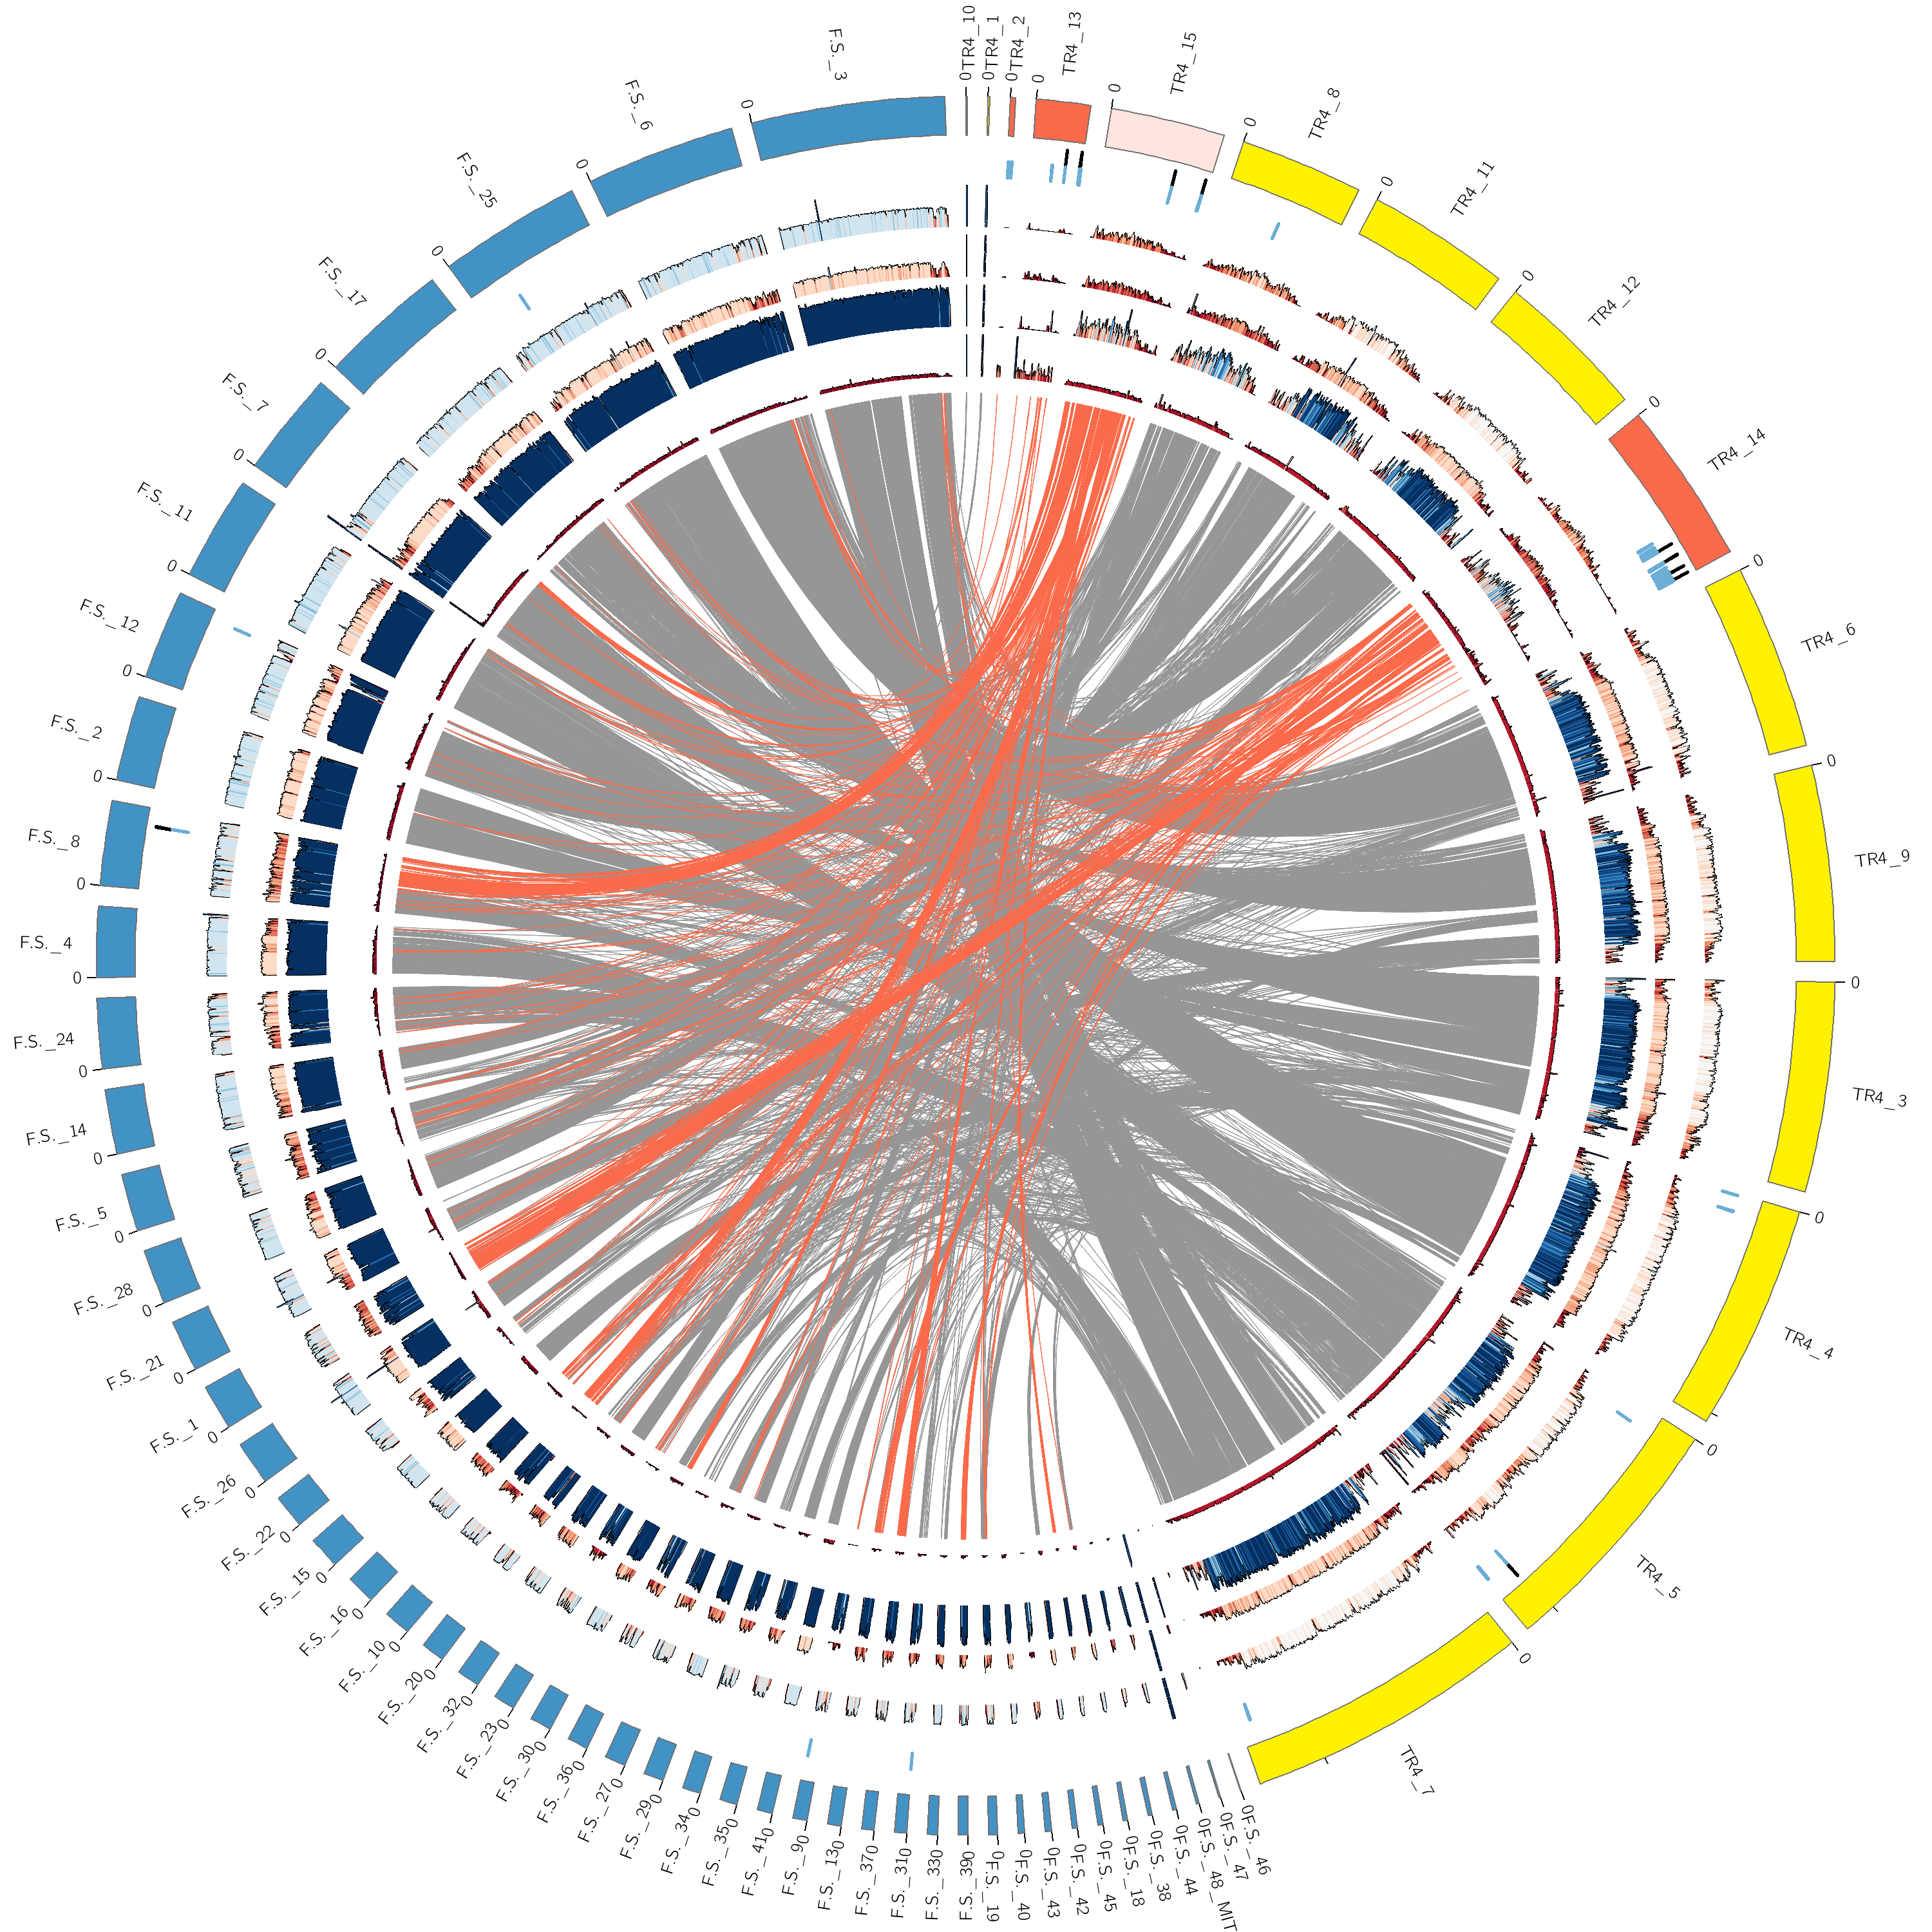
\includegraphics[width=15cm]{Figures/circos.png}
  \caption[Circos Plot of FS66 vs UK0001, including mapping data form TNAU isolates]{\textbf{Circos Plot of FS66 vs UK0001, including mapping data form TNAU isolates}}
  \label{TNAUCircos}
\end{figure}

\subsection{Results from \acf{tef} and \acf{rbp2} Phylogenies and database searches showing novel clade.}

The common Fusarium genetic barcode (Edel-Hermann and Lecomte, C., 2019) was used for phylogenetic analysis of the TNAU isolates alongside other Fusarium species. The SY-2 isolate \ac{tef} sequence extracted for the phylogeny shared in June 2022 was also included in this phylogeny for reference. For the S16 isolate, the \ac{tef} sequence was extracted from the GC-trimmed de novo assembly. For the S6 and S32 isolates, the \ac{tef} sequence was extracted from the de novo assemblies generated using all raw reads as well as the de novo assemblies generated using the reference mapped reads. 

Using a \ac{tef} database compiled from available reference sequences on the NCBI database, homologs of the \ac{tef} barcode were identified in each TNAU isolate assembly through BLASTN (1e-6 cut-off). For each assembly, the locations of hits with greater than 70\% identity and 90\% coverage were recorded, and the sequence within this region was extracted using Samtools (Version 1.15.1). Using the extracted \ac{tef} sequences the Fusariod-ID MSLT database and NCBI BLAST database were searched for similar sequences. For the S16 isolate, the Fusariod MSLT database's best scoring hits were for \ac{FFSC}, in which \textit{F. sacchari} can be found (Table: ~\ref{tab:Tef1-MLSTdb}). Further, a search of the \ac{ncbi} database revealed that the \ac{tef} sequence extracted from the S16 assembly's best scoring hits were for \textit{F. sacchari}. Searches for the S6 isolate extracted \ac{tef} sequences suggest this isolate belongs to the \ac{FOSC}. Although there were matches for \ac{Focub} \ac{tef} sequences, these were not in the top 3 results from searches of both databases for the S6 isolate. This may be due to the quality of the S6 assembly. No matches were found for the S32 extracted \ac{tef} sequences in the Fusarioid-ID MSLT database, and hits against the \ac{ncbi} GenBank database were for \textit{F. fujikuroi} isolates. 

% Please add the following required packages to your document preamble:
% \usepackage{booktabs}
% \usepackage{multirow}
% \usepackage{lscape}
\captionsetup{width=22cm}
\begin{landscape}
\begin{table}[]
\caption[\Ac{tnau} \acf{tef} \acf{ncbi} and Fusariod-ID MSLT database searches.]{\textbf{Best hits of extracted \acf{tef} sequences from the \acf{tnau} isolate \textit{de novo} assemblies against the Fusariod-ID MSLT database and \ac{ncbi} database.}}
\label{tab:Tef1-MLSTdb}
\begin{tabular}{@{}cp{3cm}p{3cm}p{3cm}p{3cm}p{3cm}p{2.75cm}@{}}
\toprule
\multirow{\textbf{\begin{tabular}[c]{@{}c@{}}TNAU Isolate \\ Assembly\end{tabular}}} &
  \multicolumn{3}{c}{\textbf{Fusariod-ID MSLT database}} &
  \multicolumn{3}{c}{\textbf{NCBI database}} \\ \cmidrule(l){2-7} 
 &
  Match 1 &
  Match 2 &
  Match 3 &
  Hit 1 &
  Hit 2 &
  Hit 3 \\ \midrule
S6 All reads &
  \ac{FOSC} &
  \ac{FOSC} &
  \ac{FOSC} &
  \begin{tabular}[c]{@{}c@{}}\textit{F. oxysporum }\\ isolate 170\end{tabular} &
  \begin{tabular}[c]{@{}c@{}}\textit{F. oxysporum }\\ f. sp. \textit{koae}\end{tabular} &
  \begin{tabular}[c]{@{}c@{}}\textit{F. oxysporum }\\ f. sp. \textit{dianthi}\end{tabular} \\
\begin{tabular}[c]{@{}c@{}}S6  \ac{Fo} \\ Mapped Reads\end{tabular} &
  \textit{\ac{FOSC}} &
  \textit{\ac{FOSC}} &
  \ac{FOSC} &
  \begin{tabular}[c]{@{}c@{}}\textit{F. oxysporum }\\ isolate 170\end{tabular} &
  \begin{tabular}[c]{@{}c@{}}\textit{F. oxysporum }\\ f. sp. \textit{koae}\end{tabular} &
  \begin{tabular}[c]{@{}c@{}}\textit{F. oxysporum }\\ f. sp. \textit{dianthi}\end{tabular} \\
S16 &
  \ac{FFSC} &
  \ac{FFSC} &
  \ac{FFSC} &
  \begin{tabular}[c]{@{}c@{}}\textit{F. sacchari} \\ CBS:147.25\end{tabular} &
  \begin{tabular}[c]{@{}c@{}}\textit{F.  sacchari} \\ NRRL 66326\end{tabular} &
  \begin{tabular}[c]{@{}c@{}}\textit{F.  globosum}\\ CBS:428.97\end{tabular} \\
S32 All reads &
  No Matches &
  No Matches &
  No Matches &
  \begin{tabular}[c]{@{}c@{}}\textit{F. fujikuroi} \\ I1.3\end{tabular} &
  \begin{tabular}[c]{@{}c@{}}\textit{F. fujikuroi} \\ IMI 58289\end{tabular} &
  \begin{tabular}[c]{@{}c@{}}\textit{F. fujikuroi} \\ Augusto2\end{tabular} \\
\begin{tabular}[c]{@{}c@{}}S32  \ac{Fo} \\ Mapped  Reads\end{tabular} &
  No Matches &
  No Matches &
  No Matches &
  \begin{tabular}[c]{@{}c@{}}\textit{F. fujikuroi} \\ I1.3\end{tabular} &
  \begin{tabular}[c]{@{}c@{}}\textit{F. fujikuroi} \\ IMI 58289\end{tabular} &
  \begin{tabular}[c]{@{}c@{}}\textit{F. fujikuroi} \\ Augusto2\end{tabular} \\
\begin{tabular}[c]{@{}c@{}}S32  \textit{F. sacchari}  \\ Mapped Reads\end{tabular} &
  No Matches &
  No Matches &
  No Matches &
  \begin{tabular}[c]{@{}c@{}}\textit{F. fujikuroi} \\ I1.3\end{tabular} &
  \begin{tabular}[c]{@{}c@{}}\textit{F. fujikuroi} \\ IMI 58289\end{tabular} &
  \begin{tabular}[c]{@{}c@{}}\textit{F. fujikuroi} \\ Augusto2\end{tabular} \\ \bottomrule
\end{tabular}
\end{table}
\end{landscape}
\captionsetup{width=0.98\textwidth}


The \ac{tef} regions from each \ac{tnau} assembly and the in-house \ac{tef} database were also used to build a phylogenetic tree. \Ac{tef} sequences were extracted from the \ac{TNAU} isolates and aligned to \ac{tef} sequences from other \textit{Fusarium} species as we as \ac{Fo} \ac{fsp}. IQ-TREE (Version 2.2.0.3) was used to infer a maximum-likelihood phylogeny using the ultrafast bootstrap setting for 1000 bootstrap replicates (Nguyen 2015). The \ac{tef} phylogeny revealed that the  S16 isolate sits within the same clade as the SY-2 isolate and reference \textit{F. sacchari} species which, taken together with the BOWTIE2 raw read mapping data, suggests these isolates may be strains of \textit{F. sacchari} pathogenic towards banana (Figure: ~\ref{fig:TEF1aPhylo}). 

The S32 isolate appears to be a sister lineage of \textit{F. sacchari}, instead, S32 grouping with the novel \textit{Fusarium} species of, \textit{F. mindanaoense}, recently reported in the Philippines by Nozawa, \et (2023) infecting Cavendish banana. The authors suggest that \textit{F. mindanaoense} is a member of the \ad{FFSC} and has acquired the \ac{sixg} \textit{SIX6}, though they have not confirmed the \textit{SIX6} homolog identified is involved in virulence in their novel species.

The S6 isolate clusters within one the \ac{Focub} clades which, alongside the higher mapping rate for to the \ac{Focub} reference and Fusariod-DB and \ac{ncbi} BLASTN results, suggests S6 is a \ac{Focub} isolate. Interestingly, based on the \ac{tef} phylogeny, S6 clusters within a \ac{Focub1} clade, but collaborators at \ac{tnau} suggest that S6 is highly virulent against Cavendish banana varieties. Due to the high amounts of contamination in the S6 raw data, it is challenging to determine the phylogenetic origin of the S6 isolate. Virulence assays comparing S6 to a \ac{r1} reference with high-quality genome sequence available, such as \ac{Focub1} strain 160527 published by Asai., \et (2019), to identify changes associated with enhanced virulence.

\begin{figure}[h!]
    \centering
    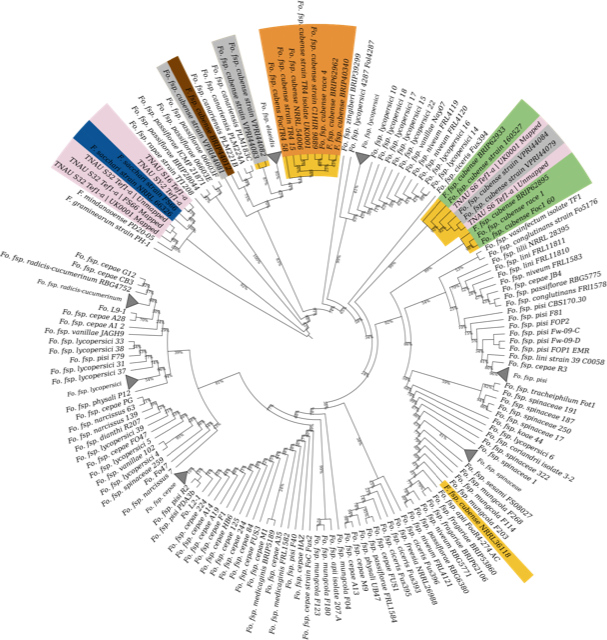
\includegraphics[width=14cm]{Figures/TEF1aPhylo-Including_mindanoense.png}
    \caption[\Acl{tef} phylogeny of \acl{tnau} \textit{Fusarium} isolates.]{\textbf{\Acl{tef} phylogeny of \acl{tnau} \textit{Fusarium} isolates.} \Ac{tnau} isolates S16, S32 and SY-2 sit within the\textit{ F. sacchari} clade. The isolates from \ac{tnau} are shown in pink. The \textit{F. sacchari} clade is shown in blue and the \acl{Focub} clades in yellow. \Acl{Focub4} isolates are in orange, and \ac{str4} in brown. \Ac{Focub} \acl{r1} isolates are shown in green. \ac{Focub} isolates from Australia with race not yet determined are shown in grey. Clades representing a single non\-\textit{cubense} \ac{fsp} have been collapsed, denoted by a grey triangle.  Percentages represent values from 1000 bootstrap replicates. The tree is rooted through \textit{Fusarium graminearum} PH-1 \ac{tef}.}
    \label{fig:TEF1aPhylo}
\end{figure}


\subsection{Ortholog analysis?}

\subsection{SIX gene searches – isolates don’t display the same SIX gene profile.}

\subsection{EffectorP outputs, any effectors which have homology to Foc predicted effectors?}


%%%%%%%%%%%%%%%%%%%%%%%%%%%%%%%%%%%%%%%%%%%%%
%DISCUSSION
%%%%%%%%%%%%%%%%%%%%%%%%%%%%%%%%%%%%%%%%%%%%%

\section{Discussion and Conclusions}
\subsection{Strength of genotyping and phenotyping – why does genotyping say it is Foc?}
\subsection{\textit{De novo} Genome Assembly and Contamination Analysis}
Using the raw reads which appear to be contaminated to generate a de novo assembly may result in misassembled contigs which are chimeric (part target species, part non-target species). These contigs can be challenging to identify and may result in contigs which should remain in the assembly being filtered out, and contigs which do not belong to the target species being kept in the assembly, even when using BlobTools to separate out target and non-target contigs. We therefore considered a reference-guided assembly approach, however, as isolates S16 and S32 have a higher mapping rate to the F. saccahri reference and assemblies generated using all raw reads contained contigs which shared greater sequence similarity with other Fusarium species, but these isolates have been classified as F. oxysporum f. sp. cubense isolates by collaborators at TNAU, determining which reference species to use it challenging. Furthermore, these isolates display a highly-virulent phenotype, and a reference-guided assembly may lose any large-scale rearrangements in the genome which may play a role in this. Consequently, for isolates S6 and S32, we have decided to map to two reference genomes (F. oxysporum f. sp. cubense TR4 isolate UK0001; F. sacchari isolate FS66) and then create a de novo assemblies with the mapped reads only. 
\subsection{High level of contamination from Stenotrophomonas.}
\subsection{Novel taxon – Similar results from Philippines paper.}

